\section{Introduction}

Compiler implementation is a complex and expensive activity~\citep{Cooper2012}.
For this reason, there has been significant interest in using machine learning
to automate various compiler tasks~\citep{Allamanis2017a}. Most works have
restricted their attention to selecting compiler heuristics or making
optimization decisions~\citep{leather2020mlinc}. Whether learned or engineered
by human experts, these decisions naturally require reasoning about the program
and its behavior. Human experts most often rely upon \textit{data flow}
analyses~\citep{Kildall1973,Kam1976}. These are algorithms on abstract
interpretations of the program, propagating information of interest through the
program's control-flow graph until a fixed point is reached~\citep{Kam1977}. Two
examples out of many data flow analyses are: \emph{liveness} -- determining when
resources become dead (unused) and may be reclaimed; and \emph{available
expressions} -- discovering which expressions have been computed on all paths to
points in the program. Prior machine learning works, on the other hand, have
typically represented the entirety of the program's behavior as a fixed-length,
statically computed feature vector~\citep{Ashouri2018}. Typical feature values
might be the number of instructions in a loop or the dependency depth. The
demonstrable weakness of these techniques is that they are trivially confused by
the addition of dead code, which changes their feature vectors without changing
the program's behavior or its response to optimizations. Such learning
algorithms are unable to learn their own abstract interpretations of the program
and so cannot avoid these pitfalls or more subtle versions
thereof~\citep{Barchi2019a}.

\begin{figure}[t]
 \centering %
 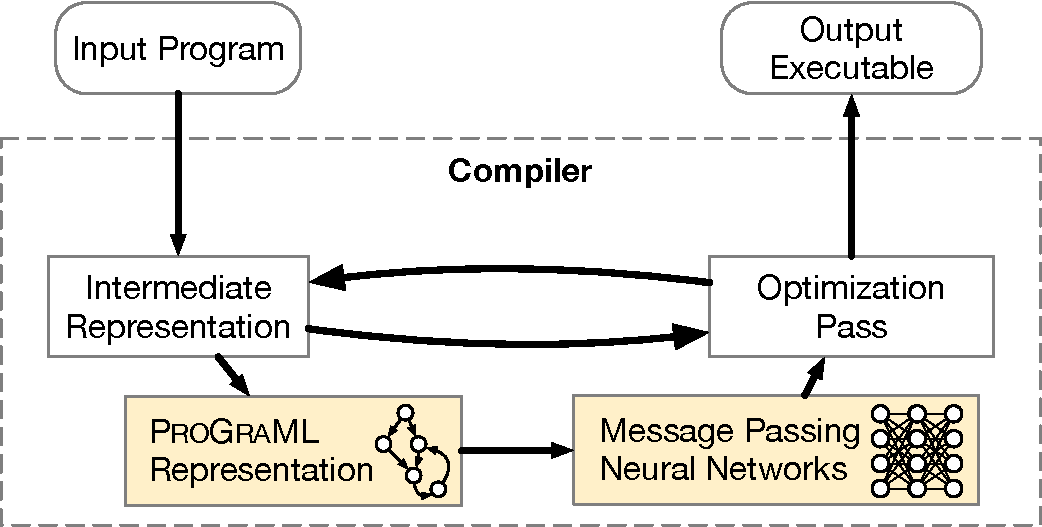
\includegraphics[width=.85\linewidth]{images/overview}
 \caption{%
    Our proposed approach for compiler analyses driven by graph-based deep
    learning.%
 }%
 \label{figure:overview}%
\end{figure}

Recently, there have been attempts to develop representations that allow
finer-grain program reasoning. Many, however, are limited both by how inputs are
represented as well as how inputs are processed. Representations based on source
code and its direct artifacts (e.g.,
AST)~\citep{Alon2018a,Yin2018,Haj-Ali2019,cummins2017synthesizing} put
unnecessary emphasis on naming and stylistic choices that may not correlate with
the functionality of the code (e.g., Fig.~\ref{subfig:code2vec}). Approaches
based on intermediate representations
(IR)~\citep{Ben-nun2018,Mirhoseini2017,Brauckmann2020} remove such noise but
fail to capture information about the program that is important for analysis
(e.g.,  Fig.~\ref{subfig:cdfg} variables, Fig.~\ref{subfig:inst2vec}
commutativity). In both cases, models are expected to reason about the flow of
information in programs using representations that do not directly encode this
information. Clearly, a program representation is needed that enables machine
learning algorithms to reason about the execution of a program by developing its
own data flow analyses.

Since current approaches are ill-suited to program-wide data flow analysis, we
propose overcoming some of their limitations by making the program's control,
data, and call dependencies a central part of the program's representation
\emph{and} a primary consideration when processing it. We achieve this by seeing
the program as a graph in which individual statements are connected to other
statements through relational dependencies. Each statement in the program is
understood only in the context of the statements interacting with it. Through
relational reasoning~\citep{Battaglia2018}, a latent representation of each
statement is learned that is a function of not just the statement itself, but
also of the (latent) representations of its graph neighborhood. Notably, this
formulation has a striking similarity to the IRs used by compilers, and the
iterative propagation of information resembles the \emph{transfer functions} and
\emph{meet operators} in traditional data flow analyses~\citep{Kildall1973}.

Recently proposed techniques for learning over graphs have shown promise in a
number of domains~\citep{Li2018a}. With a suitable representation and
graph-based model, we extend these approaches to the domain of compiler
analysis, enabling downstream tasks built on top of such graph models to
natively incorporate reasoning about data flow into their decision making. This
improves performance on downstream tasks without requiring additional features,
although challenges with respect to generalization to large programs at
test-time remain and are discussed in detail. Figure~\ref{figure:overview}
illustrates our approach. We make the following contributions:

\begin{itemize}
\item
We propose a portable, language-independent graph representation of programs
derived from compiler IRs.
\programl\footnote{\url{https://github.com/ChrisCummins/ProGraML}}
simultaneously captures whole-program control-, data-, and call relations
between instructions and operands as well as their order and data types.
\programl is a compiler-agnostic design for use at all points in the
optimization pipeline; we provide implementations for LLVM and XLA IRs.
\item
We introduce a benchmark dataset that poses a suite of established compiler
analysis tasks as supervised machine learning problems.
\textsc{DeepDataFlow}~\cite{chris_cummins_2020_4247595} comprises five tasks
that require, in combination, the ability to model: control- and data-flow,
function boundaries, instruction types, and the type and order of operands over
complex programs. \textsc{DeepDataFlow} is constructed from 461k real-world
program IRs covering a diverse range of domains and source languages, totaling
8.5 billion data flow analysis classification labels.
\item
We adapt Gated-Graph Neural Networks (GGNN) to the \programl representation. We
show that, within a bounded problem size, our approach achieves $\ge 0.939$
F$_1$ score on all analysis tasks, a significant improvement over
state-of-the-art representations. We set a new state-of-the-art on two
downstream optimization tasks for which data flow analyses are important.
\end{itemize}
